\subsection{Tunning of the parameters}


For the two MEKF methods the parametrs of the single observer was tunned first to have a good estimation of the states. Then, the parameter of the criterions computation where tunned to obtain a good rates of convergence without oscillation. For the MHE we keept de tunning of the parameters proposed in \cite{moussaDataBasedExtendedMoving2023}. \medskip

The final parameters are given here after. The Kalmant filter have been tunned using the following parameters: $P(0) = 10^{-3} \times I_{8 \times 8}$, $R_1 =  diag([5.10^{-4}, 5.10^{-4},5.10^{-4},5.10^{-4}, 1.10^{-2},  1.10^{-2}, 1.10^{-2}, 1.10^{-2}])$ , and $R_2 =  10^{5}$.\medskip

The grid of parameters choosen for the multiple observer is:

\begin{equation}
    \begin{split}
        \theta_{C_{50p}} &= [mean(C_{50p})\times [\exp^{-2std(C_{50p})}, 1, \exp^{std(C_{50p})}]] \\
        \theta_{C_{50r}} &= [mean(C_{50r})\times[\exp^{-2std(C_{50r})}, \exp^{-std(C_{50r})}, 1, \exp^{std(C_{50r})}]] \\
        \theta_{\gamma} &= [mean(\gamma) \times [\exp^{-2std(\gamma )}, 1, \exp^{std(\gamma )}]] \\
    \end{split}
\end{equation}

This choice includes the mean value which is the most probable ones, then we add the standard deviation to have a good range of values. For the lowest value the standard deviation is removed two times in order to better consider the worst cases. In fact low value for the paramters will lead to more undershoot in a close loop context. \medskip

For Petri criterion the parameters are $\lambda_1 = 0.5$, $\lambda_2 = 3$, $\nu = 10^{-5}$, and $\epsilon = 0.7$. For Narendra criterion the parameters are $\alpha = 0$, $\beta = 1$, $\lambda = 0.05$, $N = 30$, and $\epsilon = 30$.\medskip



\subsection{Results}

The results are given in the figure \ref{fig:stats_comp}. One can observe that the MEKF with the Petri criterion has the fastest convergence rates at first but then the MEKF with the Narendra criterion seems to converge to lower values. Looking at the standard deviation the Narendra criterion seems to be more stable. In those results MHE seems to be the worst option with the biggest mean value and a standard deviation comparable to the MEKF with the Petri criterion. Those results could be explained by the poor observability of the system, in fact computing the empirical grammian of the system, the minimum eigenvalue of the system is barely positive due to the low excitation of the inputs. Our guess is that the discret grid of parameter in the MEKF allow the parameters to converge faster near the true value of the parameters.\medskip 

\begin{figure}
        \center
        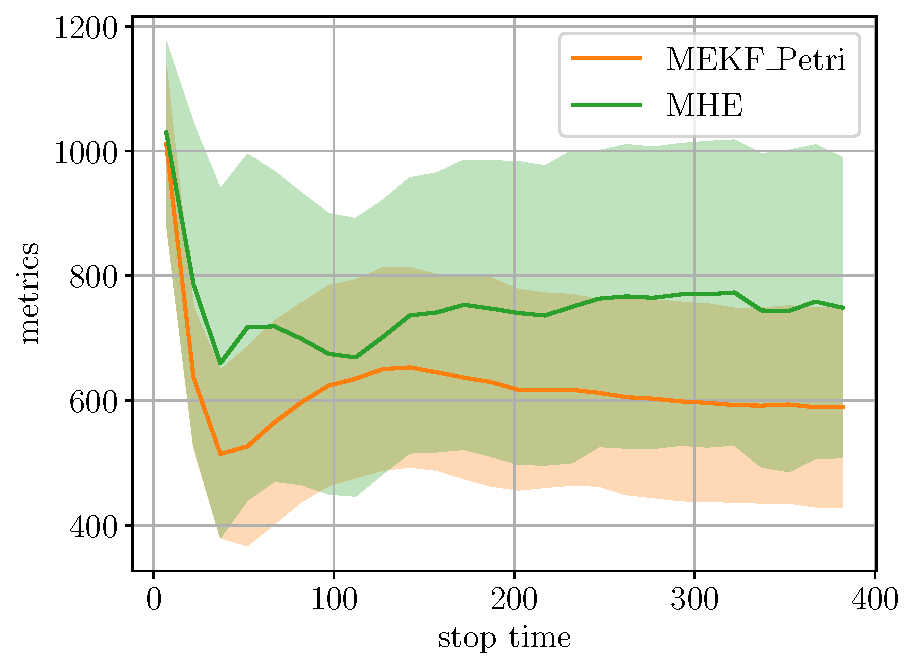
\includegraphics[width=0.7\textwidth]{../figures/stats_comp.pdf}
        \caption{Comparaison of the metrics at differents step time for the three methods. Mean value and standard deviation are given.}
        \label{fig:stats_comp}
\end{figure}


Concerning the computation times, the Petri criterion is the fastest one with a maximum computation time of 33ms for one step. The MHE is the slowest one with a maximum computation time of 425ms, and the Narendra criterion is in the middle with a maximum computation time of 271ms. All those computations time are suitable for a real time implementation as the sampling time was of 1s. This sampling time could be extended to 2s if needed.\medskip

\begin{figure}
    \center
    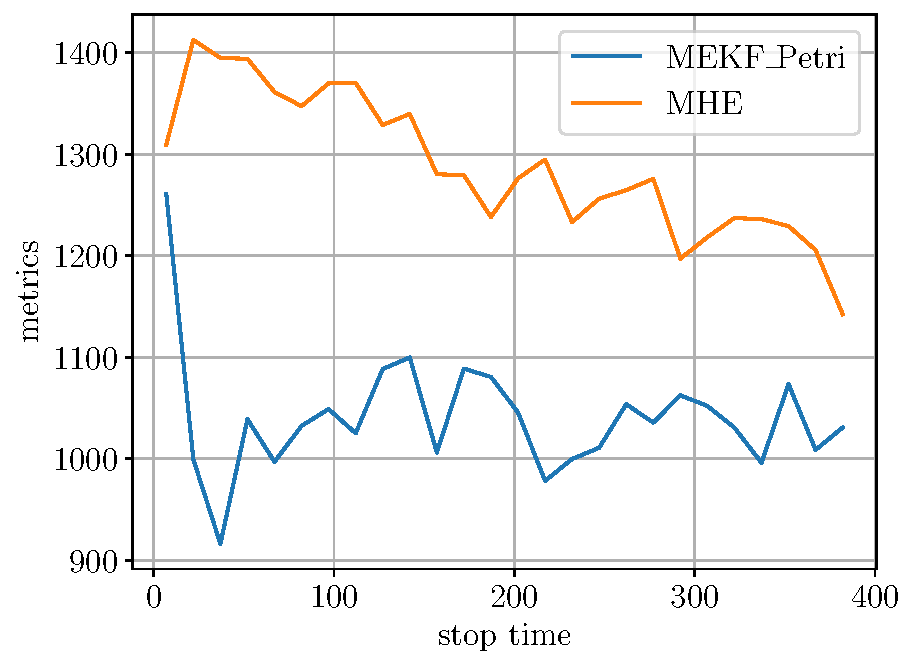
\includegraphics[width=0.7\textwidth]{../figures/stats_max.pdf}
    \caption{Maximum of the metrics at differents step time for the three methods.}
    \label{fig:stats_max}
\end{figure}

Considering the worst cases, the figure \ref{fig:stats_max} shows the maximum of the metrics for each method. One can observe that both MEKF methods leads to a constant metrics while MHE is still converging. However, the Narendra criterion reach a lower metrics while the MHE is the worst one. \medskip

All those results are very dependant of the tunning of the observer and thus must not been considered as obsolut results. However, as the tunning simplicity is also a criterion for the choice of the method, the MEKF with the Narendra criterion seems to be the best option. \medskip